% user guide(6-10 pages)
\chapter{Ръководство за потребителя}
\hfill

\section{Инсталиране на библиотеката}
        Библиотеката е съвместима с операционната система Linux. 
        Преди да започнете процеса на инсталация ще са Ви нужни следните 
        допълнителни програми:

        \begin{itemize}
                \item git
                \item Python интерпретатор (версия 3.10 или 3.11)
        \end{itemize}

        \subsection{Сдобиване с кода на библиотеката}

                Кодът на програмата може да бъде изтеглен от GitHub хранилището
                на проекта \url{https://github.com/Squidfishrl/tui-framework}.
                Най-удобният и бърз начин е да копирате хранилището директно:

                \begin{lstlisting}[style=shell]
                        $ git clone https://github.com/Squidfishrl/tui-framework
                \end{lstlisting}

                Като алтернатива може да изтеглите кода под формата на zip архив
                \figref{fig:download-zip}:
        
                \begin{figure}[h]
                \centering
                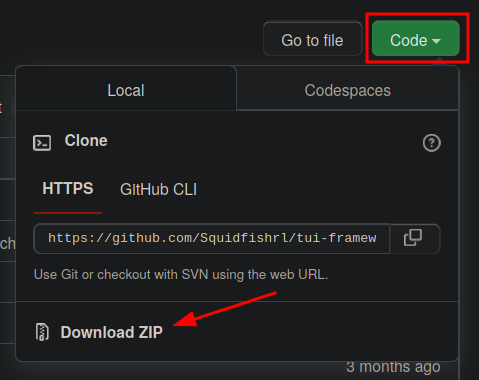
\includegraphics[width=\textwidth]{images/download-zip.png}
                \caption{Теглене на кода под формата на zip архив}
                \label{fig:download-zip}
                \end{figure}

        \subsection{Инсталиране на библиотеката}

        След като сте се сдобили с кода може да преминете към инсталацията на 
        библиотеката. Стъпките за това са следните:

        \begin{enumerate}

                \item (по желание) Създайте виртуална среда, за да изолирате
                        библиотеката от общосистемните пакети 
                        \begin{lstlisting}[style=shell]
                                $ mkdir ./venv
                                $ python3 -m venv ./venv
                                $ source ./venv/bin/activate
                        \end{lstlisting}

                \item Инсталирайте пакета
                        \begin{lstlisting}[style=shell]
                                $ pip install -e ./tui-framework
                        \end{lstlisting}



        \end{enumerate}

